\documentclass[a4paper,12pt]{article}
%%%%%%%%%%%%%%%%%%%%%%%%%%%%%%%%%%%%%%%%%%%%%%%%%%%%%%%%%%%%%%%%%%%%%%%%%%%%%%%%%%%%%%%%%%%%%%%%%%%%%%%%%%%%%%%%%%%%%%%%%%%%%%%%%%%%%%%%%%%%%%%%%%%%%%%%%%%%%%%%%%%%%%%%%%%%%%%%%%%%%%%%%%%%%%%%%%%%%%%%%%%%%%%%%%%%%%%%%%%%%%%%%%%%%%%%%%%%%%%%%%%%%%%%%%%%
\usepackage{eurosym}
\usepackage{vmargin}
\usepackage{amsmath}
\usepackage{graphics}
\usepackage{epsfig}
\usepackage{enumerate}
\usepackage{multicol}
\usepackage{subfigure}
\usepackage{fancyhdr}
\usepackage{listings}
\usepackage{framed}
\usepackage{graphicx}
\usepackage{amsmath}
\usepackage{chngpage}
%\usepackage{bigints}

\usepackage{vmargin}
% left top textwidth textheight headheight
% headsep footheight footskip
\setmargins{2.0cm}{2.5cm}{16 cm}{22cm}{0.5cm}{0cm}{1cm}{1cm}
\renewcommand{\baselinestretch}{1.3}

\setcounter{MaxMatrixCols}{10}

\begin{document}

\begin{framed} \begin{verbatim}
library(magrittr)

options(repr.plot.width=10, repr.plot.height=7)
options(digits=6)
\end{verbatim}\end{framed}


\newpage 

\begin{itemize}
    \item An exponential distribution has a parameter of $\lambda 
= 0.4$.

\item Use the in-built functions in R to perform the following tasks.
\end{itemize}




\subsection*{Exercise 1}
\noindent Simulate 1,000 values from this distribution, assigning this to a variable called ``\texttt{Exp\_Vector}`` and calculate the mean and variance of
the simulated values. Paste the results of your calculation into your answer.


\begin{framed} \begin{verbatim}
rexp(10,lambda = 0.4)
\end{verbatim}\end{framed}


\begin{verbatim}
> 
> options(digits=4)
> 
> rexp(10,lambda = 0.4)
 [1]  1.8074  1.0445  2.6367  1.2472  0.5128  1.8076
 [7]  2.0786  2.1387  4.7944 13.4485
> 
\end{verbatim}








\begin{framed} \begin{verbatim}
rexp(10,0.4)
\end{verbatim}\end{framed}

\begin{verbatim}
> rexp(10,0.4)
 [1] 8.28348 4.48688 0.86121 1.08772 0.01757 0.18649
 [7] 0.30688 1.50192 7.68903 1.86208
\end{verbatim}
%%%%%%%%%%%%%%%%%%%%%%%
\newpage
\noindent Using \texttt{set.seed()}\\
\begin{framed} \begin{verbatim}
set.seed(1234)
rexp(10,0.4)
\end{verbatim}\end{framed}

\begin{verbatim}
> set.seed(1234)
> rexp(10,0.4)
 [1] 6.25440 0.61690 0.01645 4.35687 0.96796 0.22487
 [7] 2.06020 0.50654 2.09510 1.90108
> 
> set.seed(1234)
> rexp(10,0.4)
 [1] 6.25440 0.61690 0.01645 4.35687 0.96796 0.22487
 [7] 2.06020 0.50654 2.09510 1.90108    
\end{verbatim}





%%%%%%%%%%%%%%%%%%%%%%%%%%%%%%%%%%%%%%%

\newpage 
\noindent Plot a histogram of ``\texttt{Exp\_Vector}`` showing the frequencies and paste the plot into your answer.

\begin{framed} \begin{verbatim}
set.seed(1234)
Exp_Vector <- rexp(1000,0.4)
\end{verbatim}\end{framed}


\begin{framed} \begin{verbatim}
mean(Exp_Vector) 
\end{verbatim}\end{framed}


2.50153343647035



\begin{framed} \begin{verbatim}
mean(Exp_Vector) %>% round(3)
\end{verbatim}\end{framed}


2.502



\begin{framed} \begin{verbatim}
summary(Exp_Vector)
\end{verbatim}\end{framed}


         Min.   1st Qu.    Median      Mean   3rd Qu.      Max. 
     0.000592  0.712687  1.792930  2.501533  3.467425 18.167711 



\begin{framed} \begin{verbatim}
var(Exp_Vector) %>% round(3)
\end{verbatim}\end{framed}


6.393

\begin{itemize}
    \item The mean and variance will vary due to the random number generation. 

If the sample size was large enough, the mean and variance should be close the underlying distribution (exponential with parameter 0.4) as follows:

Mean = 2.5

$$ E(X) = \frac{1}{\lambda} = 2.5$$

Variance = 6.25

$$ \operatorname{Var}(X) = \frac{1}{\lambda^2} = 6.25$$
\end{itemize}


%%%%%%%%%%%%%%%%%%%%%%%%%%%%%%%%%%%%%%%%%%%%
\newpage
\noindent Plot the probability density function for this distribution as:

1. a scatter plot
2. a line graph.



\begin{framed} \begin{verbatim}
hist(Exp_Vector)
\end{verbatim}\end{framed}


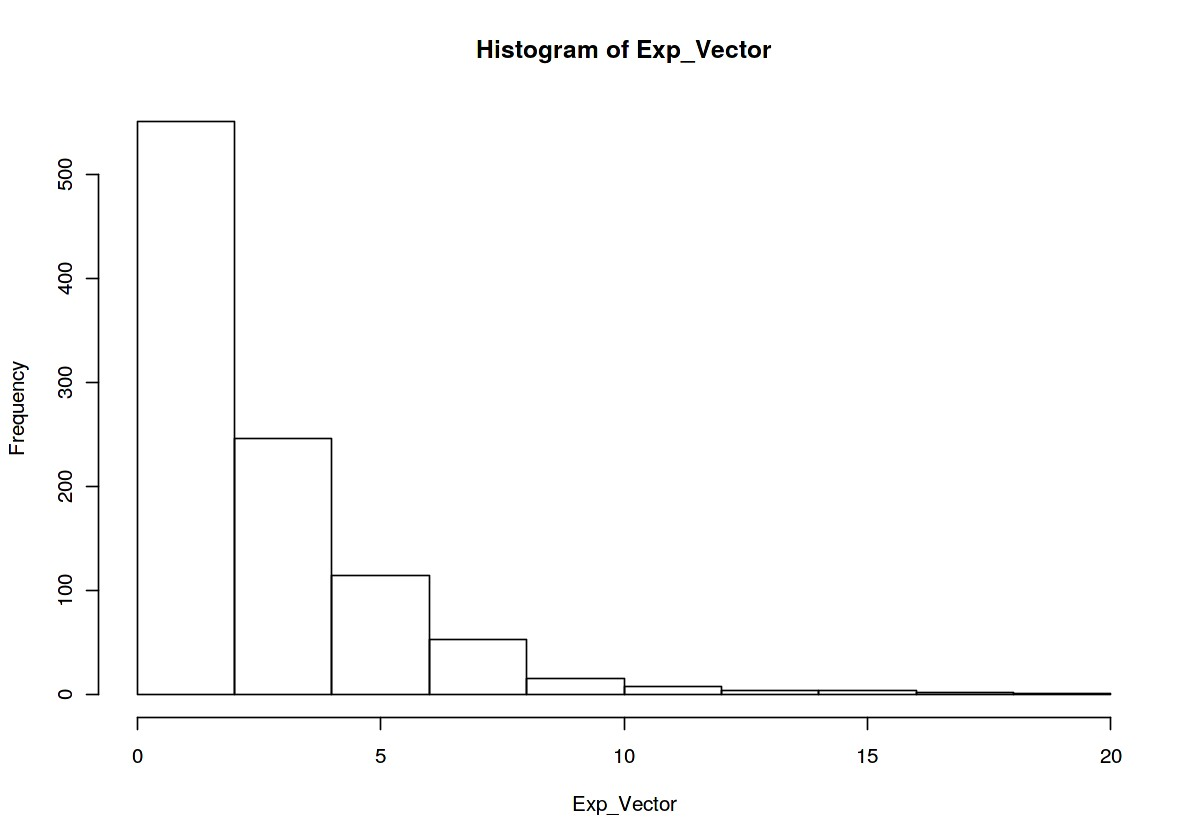
\includegraphics[scale=0.400]{00-A2/images/output_13_0.jpeg}



\begin{framed} \begin{verbatim}
hist(Exp_Vector, breaks=50,col=c("lightblue","pink"))

\end{verbatim}\end{framed}

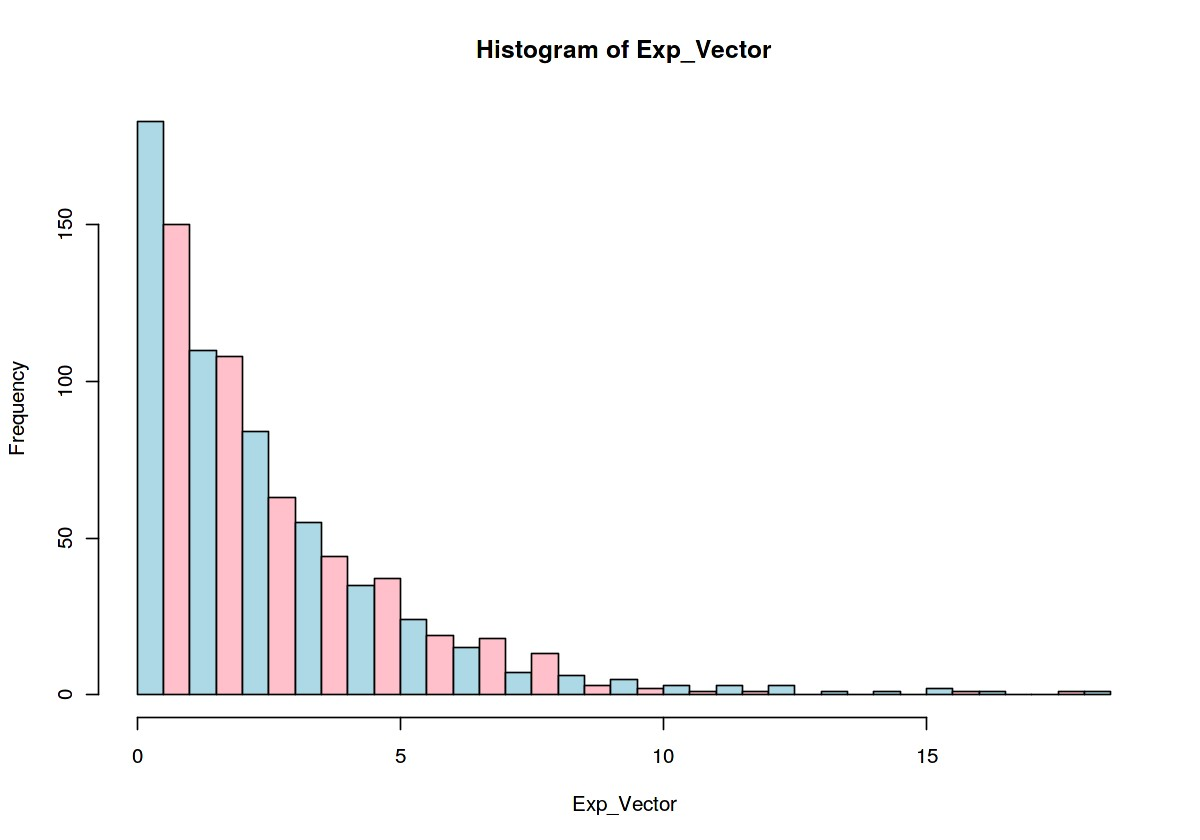
\includegraphics[scale=0.40]{00-A2/images/output_14_0.jpeg}

%%%%%%%%%%%%%%%%%%%%%%%%%%%%%%%%
\newpage 

\begin{framed} \begin{verbatim}
x <- seq(0,20,by=0.5)
x
\end{verbatim}\end{framed}

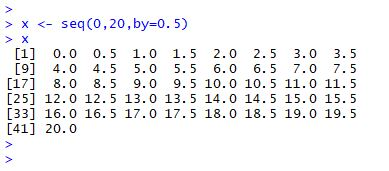
\includegraphics[]{00-A2/images/Sequence.JPG}

\newpage 

\begin{framed} \begin{verbatim}
PDF <- dexp(x, 0.4)

plot(x, PDF)

\end{verbatim}\end{framed}


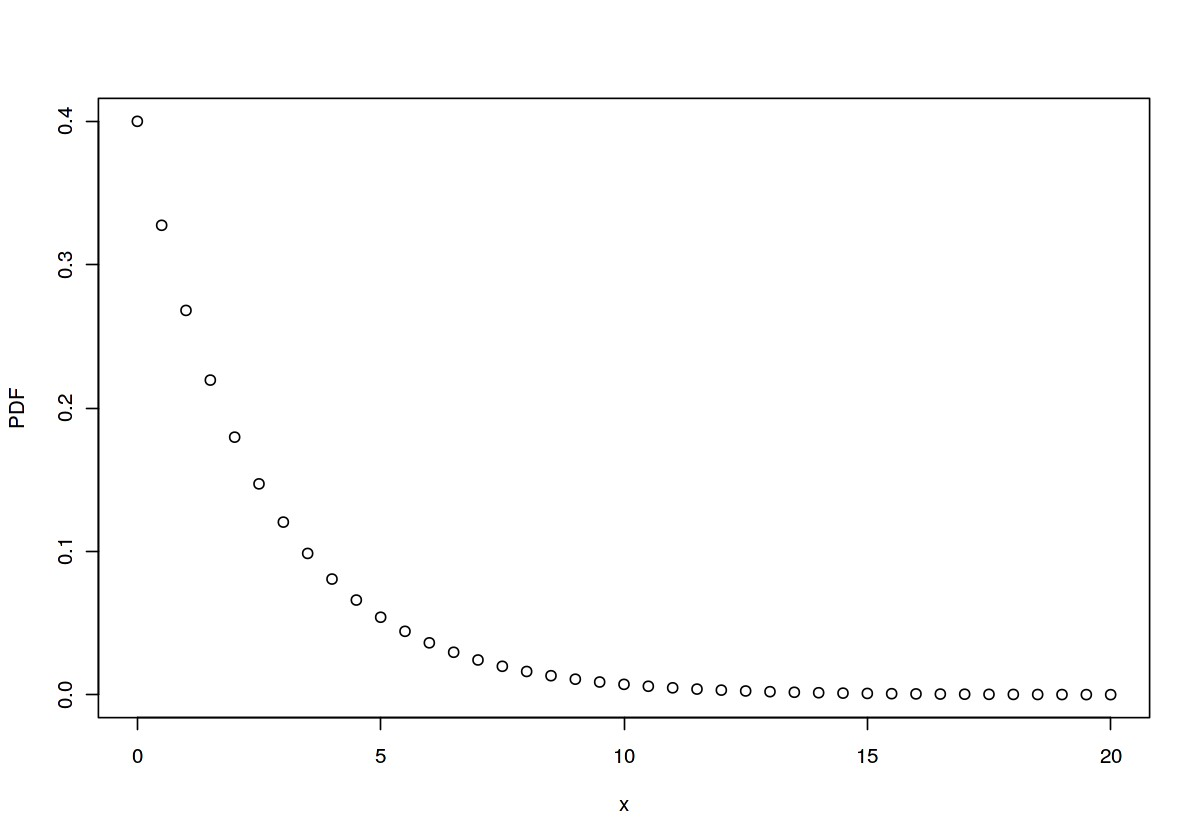
\includegraphics[scale=0.4]{00-A2/images/output_16_0.jpeg}

\newpage 

\begin{framed} \begin{verbatim}
plot(x, PDF, type="l")
\end{verbatim}\end{framed}


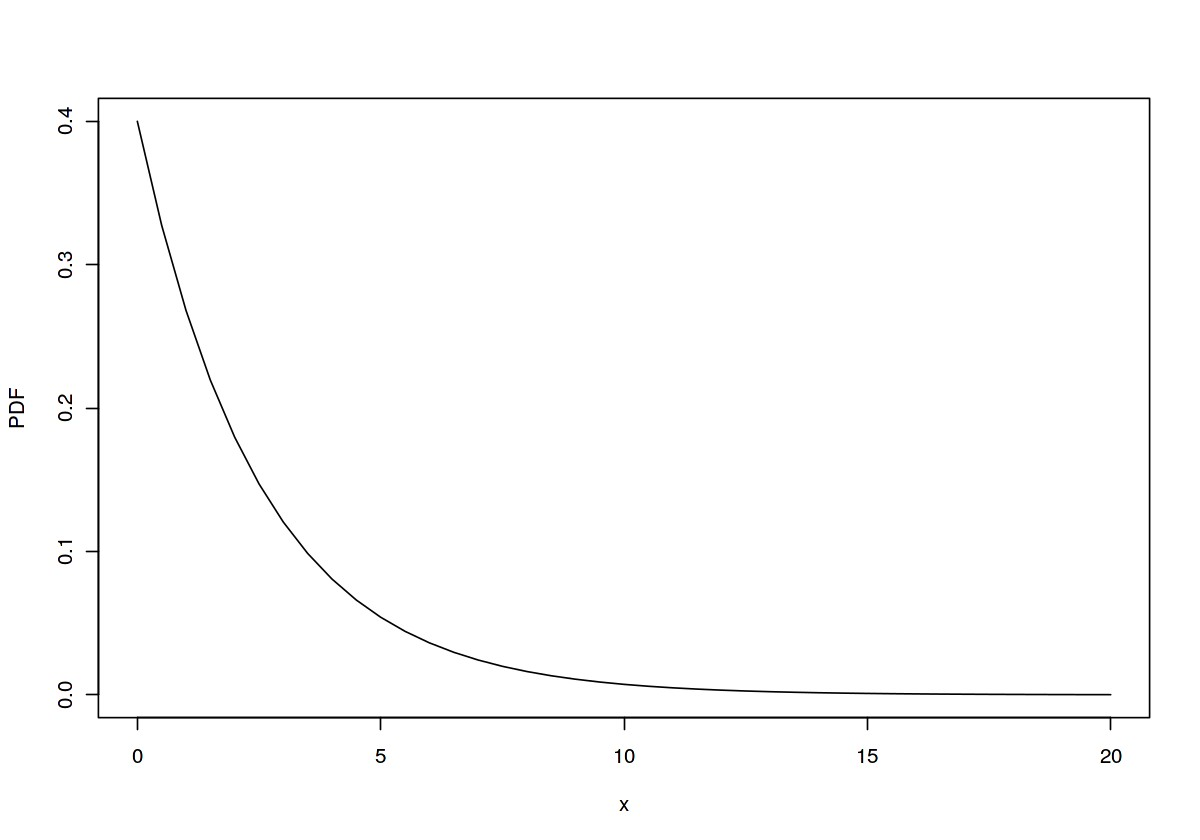
\includegraphics[scale=0.4]{00-A2/images/output_17_0.jpeg}

%%%%%%%%%%%%%%%%%%%%%%%%%%%%%%%%%%%%%%%%%%%%%%%%%%%%

\newpage 
\subsection*{Exercise  2}

A lognormal distribution has parameters $\mu = 0$ and $\sigma^2 = 1$.

%Use the in-built functions in R to:
% subsubsection*{Task a}

\noindent Simulate 1,000 values from this distribution, assigning this to a vector called ``\texttt{LNorm\_Vector}`` and calculate the mean and variance of the simulated values. 




\begin{framed} \begin{verbatim}
set.seed(1234)
LNorm_Vector <- rlnorm(10000, meanlog = 0, sdlog = 1)
\end{verbatim}\end{framed}
\begin{framed} \begin{verbatim}
mean(LNorm_Vector) 

var(LNorm_Vector) 
\end{verbatim}\end{framed}


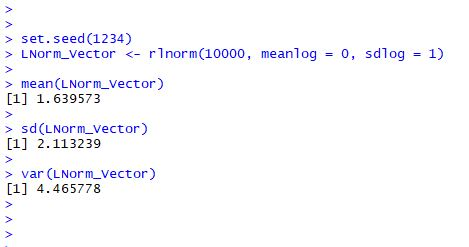
\includegraphics[scale=1.2]{00-A2/images/lognormal_1_estimates.JPG}

\begin{itemize}
    \item The mean and variance will vary due to the random number generation. 

\item If the sample size was large enough, the mean and variance should be close the underlying
distribution (lognormal with parameters $ \mu = 0$, $\sigma^2 = 1$) as follows:\\
Mean = 1.649\\
Variance = 4.6708\\
\end{itemize}

\newpage 

Plot a histogram of ``\texttt{LNorm\_Vector}`` showing the frequencies.



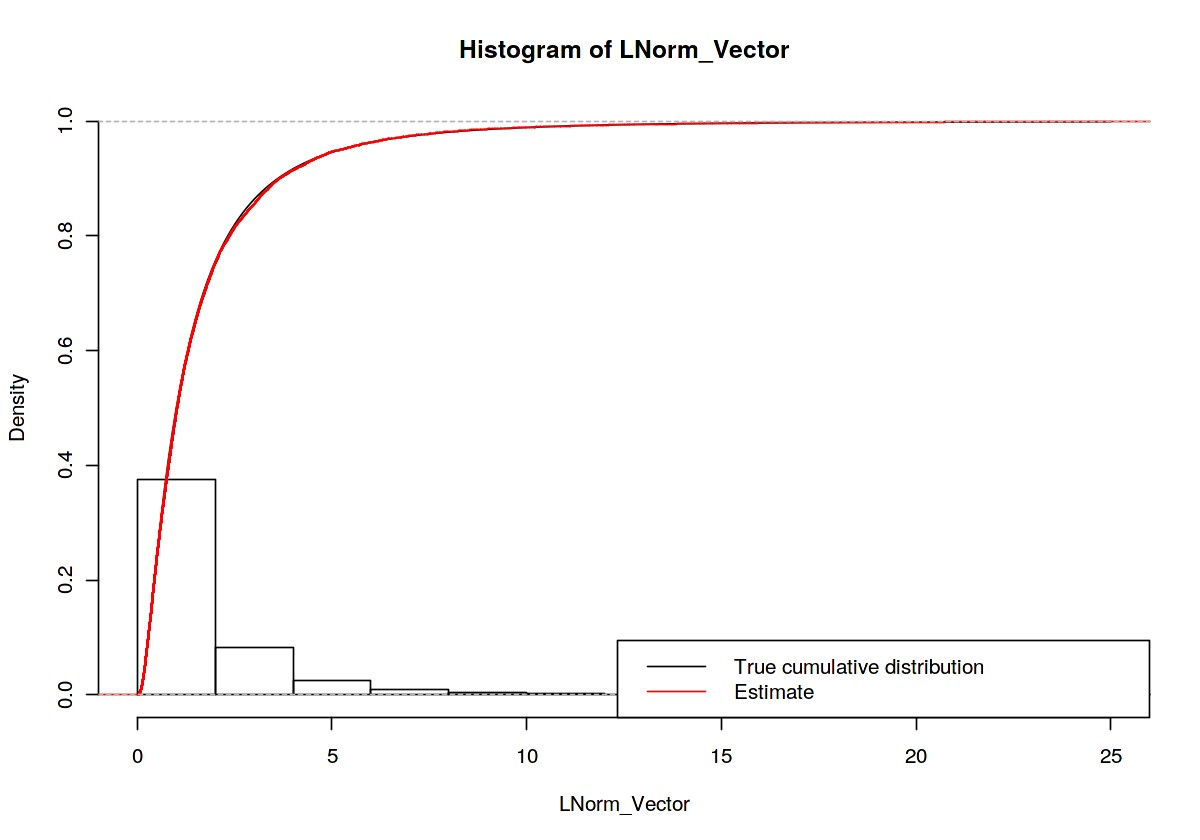
\includegraphics[scale=0.4]{00-A2/images/output_23_0.jpeg}

%%%%%%%%%%%%%%%%%%%%%%%%%%%%%%%%%%%%%%%%%%%%%%%%
\newpage 
\subsection*{Task (c)}

Plot a second histogram in a new graph of ``\texttt{LNorm\_Vector}`` showing the probability densities, setting the y-axis range from 0 to 0.7 for this graph.


\begin{framed} \begin{verbatim}
hist(LNorm_Vector, breaks=25, freq = FALSE, xlim = c(0,25), ylim = c(0,1))

grid = seq(0,25,0.1)
lines(grid, plnorm(grid,0,1),type="l",xlab="x",ylab="f(x)", col="black")
lines(ecdf(LNorm_Vector),col="red")
legend("bottomright",c("True cumulative distribution","Estimate"),lty=1,col=c("black", "red"))
\end{verbatim}\end{framed}




\begin{framed} \begin{verbatim}
hist(LNorm_Vector)
\end{verbatim}\end{framed}


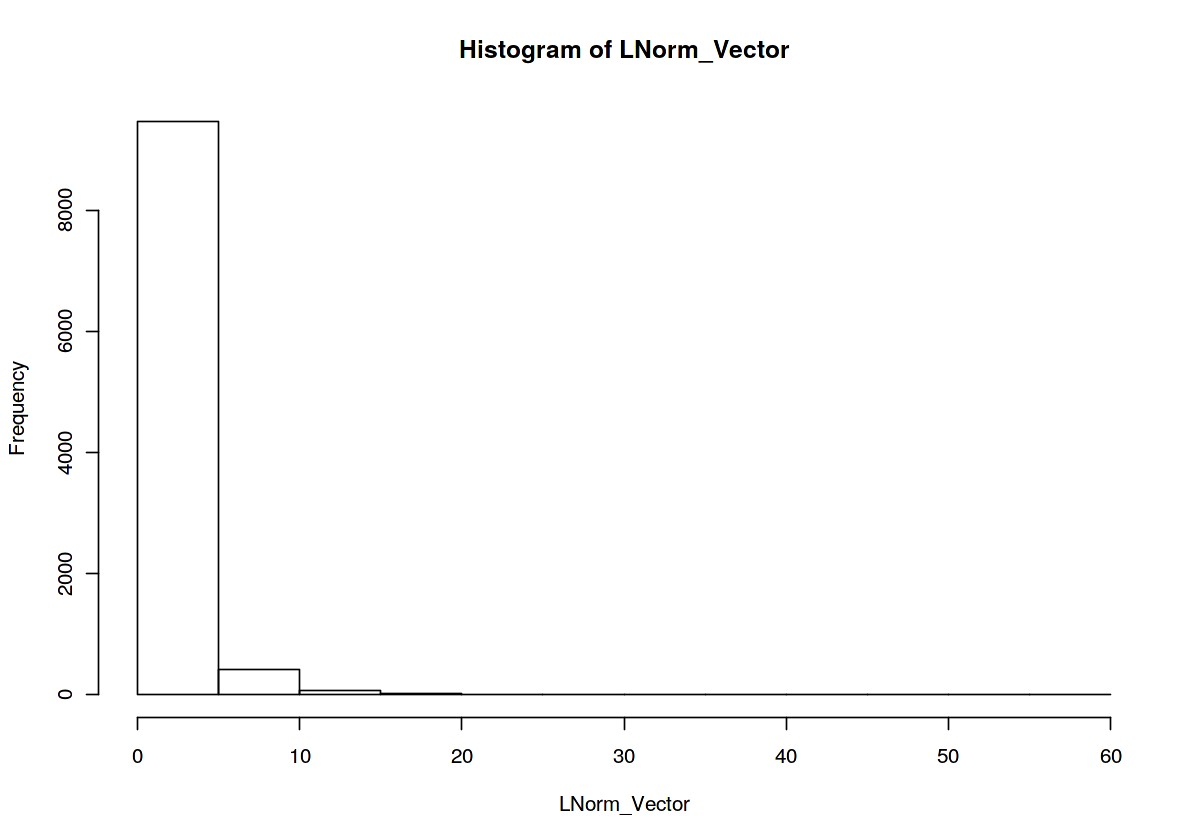
\includegraphics[scale=0.4]{00-A2/images/output_24_0.jpeg}




\begin{framed} \begin{verbatim}
hist(LNorm_Vector, freq = FALSE, xlim = c(0,25), ylim = c(0,0.7))
\end{verbatim}\end{framed}


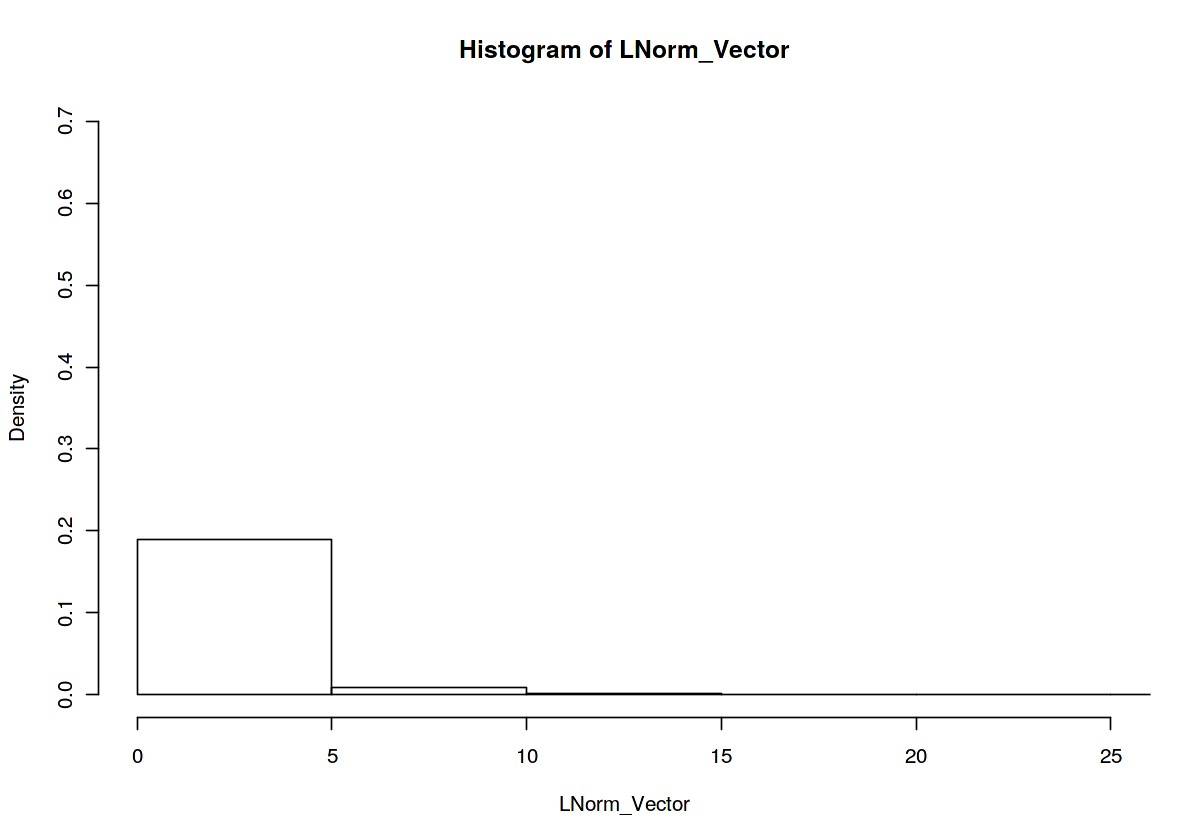
\includegraphics[scale=0.4]{00-A2/images/output_25_0.png}

%%%%%%%%%%%%%%%%%%%%%%%%%%%%%%%
\newpage 

%%#### Exercise  (d)
Add the cumulative density function of \texttt{LNorm\_Vector} to the chart
in Exercise  (ii)(c) and paste the plot into your answer.

%%#### Exercise  (e)

Add the theoretical lognormal (0,1) distribution to the chart in Exercise  (ii)(d) to highlight the difference to the sample, including
appropriate labels and legend and paste the plot into your answer.

%%


\begin{framed} \begin{verbatim}
lines(grid, dlnorm(grid,0,1),type="l",xlab="x",ylab="f(x)", col="black")

lines(density(LNorm_Vector), col="red")

legend("topright",c("True Density", "Estimate"),lty=1,col=c("black", "red"))

\end{verbatim}\end{framed}


%%%%%%%%%%%%%%%%%%%%%%%%%%%%%%%%%%%%%%
\newpage 



The output is:
(iii) (a)

\begin{framed} \begin{verbatim}
rpareto <- function(n,alpha,lambda) {
rp <- lambda*( (1-runif(n))^(-1/alpha) -1 )
rp
}
\end{verbatim}\end{framed}


\begin{framed} \begin{verbatim}

LNorm_Vector = rpareto(1000, 3, 1)
mean(LNorm_Vector)
var(LNorm_Vector)
\end{verbatim}\end{framed}



The mean and variance will vary due to the random number generation. If the sample size
was large enough, the mean and variance should be close the underlying distribution
(Pareto α = 3, λ = 1) as follows:
Mean = 0.5
Variance = 0.75

\newpage 
%%%%%%%%%%%%%%%%%%%%%%%%%%%%%%%%%%%%%%%%%%%%%%%55
Note: The correct R code receives full marks.
Candidates are not required to paste theirs simulated sample.
Note: Alternative solutions to (iii) are possible. For example,
\begin{framed}
\begin{verbatim}
rpareto <- function(alpha, lambda) {
rp <- lambda*( (1-runif(1))^(-1/alpha) -1 )
rp
}
LNorm_Vector = replicate( 1000, rpareto(3,1)
mean(LNorm_Vector)
var(LNorm_Vector)
)
\end{verbatim}
\end{framed}

%Note: Some candidates may use something equivalent to Pareto_Vector rather than LNorm_Vector.
%Marks should not be deducted for this.
%This question was answered well by most candidates.

\end{document}
